\documentclass[pdftex,a4paper,14pt,english]{extarticle}

\usepackage[top=2cm,bottom=27mm,left=3cm,right=18mm]{geometry}
\usepackage[utf8]{inputenc}
\usepackage[english]{babel}
\usepackage[pdftex]{hyperref}
\usepackage{indentfirst}
\usepackage[pdftex]{graphicx}
\usepackage{amsmath}
\usepackage{amssymb}
\usepackage{ragged2e}
\usepackage{multirow}
\usepackage{array} % for defining a new column type
\usepackage{varwidth} %for the varwidth minipage environment
\usepackage{algorithmic}
\usepackage[boxed]{algorithm}
\usepackage{tabularx}
\usepackage{xtab}
\usepackage{subfig}
\usepackage{hyphenat}
\usepackage{setspace}
\usepackage{fancyhdr}
\usepackage{tikz}
\usepackage{pgf-umlsd}
\usepackage[toc,page]{appendix}
\usepackage{listings}
\usepackage{wrapfig}
\usepackage{chngcntr}
\usepackage{csvsimple}
\usepackage{pgfplotstable,filecontents}

\pgfplotsset{compat=1.9}% supress warning



\counterwithin{figure}{section}

\usetikzlibrary{arrows}
\usetikzlibrary{positioning,fit,calc}
\usetikzlibrary{shapes,snakes}
\usetikzlibrary{calc,trees,positioning,arrows,chains,shapes.geometric,
    decorations.pathreplacing,decorations.pathmorphing,shapes,
    matrix,shapes.symbols}


\pagestyle{fancyplain}
\fancyhf{}
\renewcommand{\headrulewidth}{0pt}
\rfoot{\fancyplain{}{\thepage}}

\linespread{1.15}
\floatname{algorithm}{Algorithm}

\addto\captionsrussian{\renewcommand{\contentsname}{Content}}

% new commands
\newcommand\sign[1]{sign(#1)}
\newcommand{\includecode}[2][c]{\lstinputlisting[caption=#2, escapechar=, style=custom#1]{#2}}

\begin{document}

\newcolumntype{M}{>{\begin{varwidth}{4cm}}l<{\end{varwidth}}} %M is for Maximal column

\setcounter{page}{1}
\tableofcontents

\newpage

\section{Introduction}
\addcontentsline{toc}{section}{Introduction}

\subsection{Background}

The thesis project is done in the company \textit{Accedo Broadband AB}. \textit{Accedo is the market leading enabler of TV application solutions. Accedo provides applications, tools and services to media companies, consumer electronics and TV operators globally, to help them deliver the next-generation TV experience. Accedo’s cloud-based platform solutions enable customers to cost-efficiently roll out and manage application offerings and stores for multiple devices and markets} \cite{Accedo}.

The main business of the company is developing smart user applications for customer APIs. Unfortunately, every customer API was developed in a unique way and has their own communication protocol. Consequently, it is difficult to write smart user applications that use many customer APIs because a developer would have to write the communication layer for every customer API. 

The problem can be defined as follows:  There are a lot applications written for different operating systems and they require frequent communication with many customer APIs. What architecture is the most appropriate for communication between applications and external services represented by a customer APIs? 

One of the solutions, is a simple direct communication between client and services. The client will send requests to every service and wait for responses. This solution has several drawbacks: a developer would have to maintain many communication layers written in different languages. When the external API changes, the developer would be forced to rewrite every communication layer. This increases the cost of development and the development time. Another problem is security, some services might have a private API that should not be used directly.

A different solution will be to introduce the middle layer between the client and external services. The client will communicate with middle layer using predefined protocol, middle layer will then gather data from external services and send it to the client. This approach has several benefits: every application will be written with standardised communication API, defined by the middle layer; if external API changes, only middle layer should be rewritten; the response time can be decreased by caching the data in the middle layer. 

Another solution can be the usage of CDN (Content Delivery Networks). The application will send the requests directly to the external services, but the request will be intercepted and handled by the CDN Edge Servers that are located between Application and External Services. This solution requires dynamic usage of HTTP Cache-Control headers. The advantage of using CDN is that the developer need not maintain the middleware service. Alternatively, the results will be cached somewhere on the way between Application and External services producing a faster response to the final user. On the other hand, the drawbacks are that it is difficult to configure CDN to process dynamic content and the developer would need to write the communication layer for every external service. 

This project tries to break the connection between applications and external services by providing the middle layer. The applications communicates with the middleware using a predefined format that is the same for every platform. The middleware will manage the requests, translate them to the format appropriate for the external services and forward them to the appropriate servers. It will also manage the responses from servers and send them back to the applications.


\subsection{Project Objectives}

The project is in the context of networking, caching and data aggregation. The goal of the project is to investigate different solutions for implementing a caching layer used in a backend middleware, design and develop prototypes for each solution, run set of tests and select the most optimal solution.
The selected solution is then further developed and integrated into an existing middleware provided by the company, and an analysis is then made in a real life scenario.


\subsection{Thesis Outline}

During the project the middleware server developed by company will be examined. The application will be studied and analysed in development environment. The set of problems and future improvements will be retrieved and discussed. The appropriate solutions for selected problems will be presented in this paper.

The Theory section will give the information about the modern web caching technologies and how they can be used on practice. Also, some parts of HTTP protocol will be introduced.

The Architecture overview will present the company solution and will identify the drawbacks. The web caching solution for some problems described in architecture overview will be introduced.

The HVG chapter will present the second part of the thesis: Hierarchical VMO Generator.

The Test chapter will compare the performance of Redis cache and Web cache solutions and evaluate the HVG algorithm in comparison with existing solution.

\newpage

%TODO investigate the code repositories
%TODO define the common pattern for the server interaction
%TODO define request/response types(what can be combined, what cannot) for client part
%TODO update the report, add information about types to the server achitecture, introduce new problem if exists 
%TODO Make dependencies to the json tree*
%TODO update report with the algorithm of request aggregation 
%TODO integrate json tree* to the VIA app
%TODO update the report, add information about integration
%TODO set the web cache with for the dynamic and static content between via and clients
%TODO set the web cache between via and ovp
\section{Theory}
	
\subsection{Content Delivery Networks}


Nowadays the Internet is available almost from any place in the world. It allows people from different countries to communicate with each other and exchange information. The content providers and applications should serve the user's requests from all around the world with the equally high speed in order to provide good user experience. For solving this task, companies should deploy their servers all around the world in multiple data centers. For world-class companies like Google and Netflix this task is solvable\cite{NetflixCDN}, but for middle sized companies there should be another solution because it is very expensive and sometimes complicated to deploy servers in multiple data centers. Fortunately, the content delivery networks solve this problem\cite{AkamaiCDN}.

The Content Delivery Network(CDN) is a distributed system consisted of many servers deployed all around the world in different data centers. They act as a local content holders. The routes to the content providers and applications are configured to lay through the CDN's servers. When the client wants to access the server through the Internet the request will be processed by the local CDN server and if it will find the data locally, it will deliver the response to the client without making the request to the content provider that can be located in different country. The CDNs can store both static and dynamic content. One of the first global solutions was presented by Akamai company\cite{AkamaiCDN}. The graphical architecture is depicted on figure \ref{fig:cdn_overview}.

The CDN consists of several parts: routing, load balancing and web caching\cite{CDNOverview}. The web caching part will be reviewed because it is relevant to the project.

\begin{figure}[h]
    \centering
    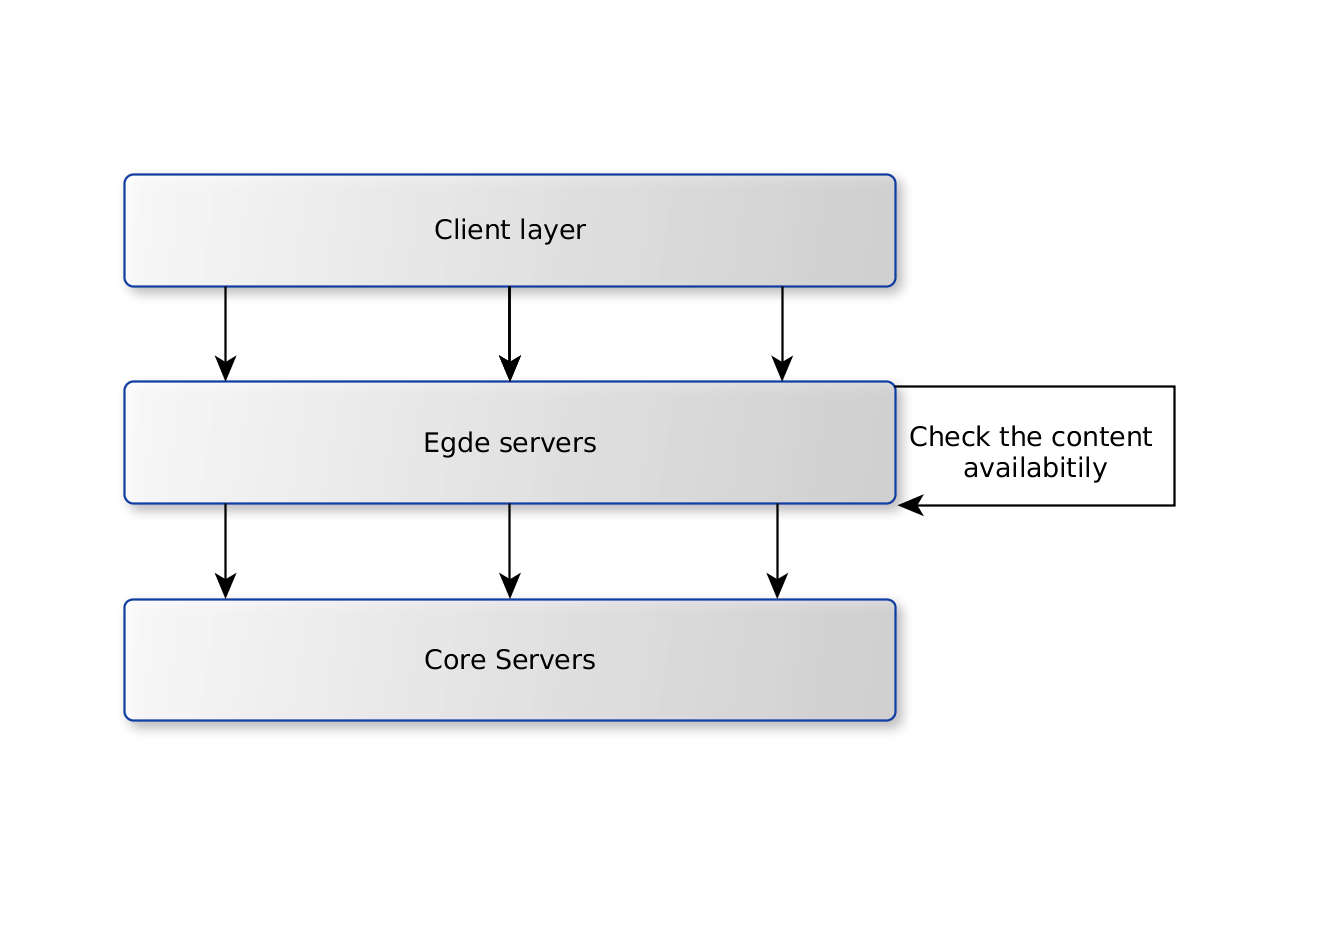
\includegraphics[width=\textwidth]{images/cdn_arch.png}
    \caption{Content Delivery Network Overview}
    \label{fig:cdn_overview}
\end{figure}

\subsection{Web Caching}

Web caching is the technique that allows to store temporary content that is requested from the Internet e.g. HTML pages, JSON, XML or CSS files. It alleviates the server's work by reducing the amount of requests to it and reduces bandwidth usage\cite{WebCachingInterior}. A web cache system serves as a communication point between client and sevrer. The client's requests and server's responses are routed through it. The web cache stores responses from the server and returns them without hitting the underlying server. It also can manipulate the request/response headers.

The benefits of web caching:

\begin{itemize}
    \item Reduces the server workload. Using web caching the requests will go through the cache and will touch server only if the data does not present in caches or the data is stale. That will reduce the amount of requests made to server.
    \item Web caching improves user experience. The data will be delivered faster to the end users.
    \item Reduces bandwidth
\end{itemize}

\subsubsection{Content types}

% Describe static and dynamic content types

The content stored by web caches can be static or dynamic.

The static content is a set of resources that stay the same no matter what was the user input. Static objects are identified by the unique path and can be cached for a long time by the web caches.

The dynamic content is generated at run-time, based on the user input\cite{DynamicWebCaching}. The dynamic requests almost always processed by severs. They are the main consumers of the web server's resources. The dynamic requests are time dependant meaning that in different time the same request can produce different output, as a result they cannot be cached for a long time by the web caches. Moreover, for security reasons, usually dynamic objects that contain client's personal data and preferences are configured in order not to be cached by the external web caches and CDNs.

However almost all dynamic content is static for a short period of time. It changes only when the internal resouces e.g. databases are altered. This gives a possibility to configure web cache for storing dynamic objects.

\subsubsection{Http Cache Control Headers}

Web cache is controlled by the http cache control headers\cite{RFC7234}. The control mechanisms can be specified on both request and response sides. There are several http headers that are relevant for the project: 
\begin{itemize}
    \item Cache-Control
    \item Vary header
    \item Etag, If-None-Match
    \item Last-Modified, If-Modified-Since
    \item Expires( for http 1.0 )
    \item Widely used extension headers, like X-Cache.
\end{itemize}

There are two caching techniques: Time based caching and Data based caching.

The time based caching is represented by the next http headers: \textit{Last-Modified} and \textit{If-Modified-Since}, \textit{Cache-Control} with \textit{s-maxage} parameter and \textit{Expires} header. Client sends the request with specified \textit{If-Modified-Since} header, where he indicates as a parameter the time when the content was modified. The server will check the type of the content which was requested and send the corresponding response. If the static content was requested, the server will check if the resource was changed since the date specified by the client in \textit{If-Modified-Since} header, and will send the new content with the code 200 and updated \textit{Last-Modified} header if it was modified, otherwise it will reply with the code 304(resouce not modified) without content and with old \textit{Last-Modified} header. The server usually does not set the Last-Modified header to the dynamic resources because it is hard to know where exactly they were modified. 
During the response the server can specify the \textit{Cache-Control} header with s-maxage parameter. In this case, if the content is public, it can be cached by the web cache servers for s-maxage time specified in seconds. If the next request will occur in the next \textit{s-maxage} seconds, the content will be served from the web cache. This technique is used for caching both dynamic and static content. The difference between static and dynamic content is that the s-maxage parameter fot the dynamic content is set dynamically, and it is static for the static content.(change the last sentence)

The data based caching is represented by the \textit{Etag} and \textit{If-None-Match} headers. It is supported since in HTTP/1.1. On the first request the server will compute the hash of the content and send it to the client in the Etag header. The client will remember the hash value in the \textit{If-None-Match} header. When the next request occurs, the server will recompute the hash of the content and will compare it with the value specified in the If-None-Math parameter. If the values are the same, the server will reply with the 304 code, without content and with the old Etag header, otherwise it will change the Etag header to the new value and send the normal response. 


The web cache can be implemented on: 

\begin{itemize}
    \item Client side, by using browser caches
    \item Proxy servers, by introducing the middle caching server between client and server.
    \item Server side, by implementing cache programmatically
\end{itemize}

Currently, the middleware server supports the server side caching with Redis in memory data store. We will introduce the proxy server caching and will see if it will give the benefit to the architecture.(move to abstract) 

\subsubsection{An overview of proxy server types}

A proxy server is a server that is deployed between client and server. It serves as a middle point in communication between clients and servers. The proxy server redirects requests to servers and responses from servres. It can improve the performance of the servers by storing the copies of frequently used resources. When a client makes a request to the server through the proxy server, the  proxy server serves as a web cache, it will try to find data locally and will return the resource back to the client on success.

There are two main types of proxy servers: forward and reversed proxy\cite{WWWCaching}.
A forward proxy is a one of the most common types of proxy servers. The client is aware about the proxy server and can configure requests through it.
A reversed proxy is deployed by server administrators in the internal network. The client contacts the desired server, but the request is routed through the reversed proxy server. In this case, the client may not know about the underlying proxy. 
The reversed proxy server was selected for the project because it perfectly suits the architecture, the client should not know about the existence of the middle point. (and the web caching is mostly done by using reversed proxy servers).


\subsection{Http Session Management}

HTTP protocol is stateless by its nature, meaning that there is no possibility to distinguish one request from another. Http requests usually open new connection to the desired server every time. Nowadays, server can specify \textit{Keep-Alive} header in the response in order to give browser a hint that this connection can be used again for the new request. Unfortunately, without transferring user-specific information it is impossible to distinguish users.  

The session management is implemented through header fields  \textit{Set-Cookie} and \textit{Cookie} headers. When server wants to distinguish one user from another it sets the unique identifies for the user. This identifier is transferred in the header field Set-Cookie. The browser will parse this field and remember the unique identifier. For every new request, browser will send this identifier it header field Cookie. Of course server can send additional information in Set-Cookie header, that is unique for user. Unfortunately, it is very dangerous to transfer private information(e.g. credit card number) this way. The server can store dictionary of user ids and corresponding private information in memory and retrieve this information every time when the browser specifies Cookie header. 


\newpage



% \section{Architecture Web}

\subsection{HTTP Protocol}

\subsection{SPDY Protocol}

\subsection{Web Caching Architecture}

\newpage

\section{Middleware Architecture}

\subsection{Server Architecture}

The company architecture contains the following components: Client Application, Middleware server, Middleware Cache, Metadata Server, and Content Servers. The brief architecture overview is presented on figure \ref{fig:arch_overview}. 


\begin{figure}[h]
    \centering
	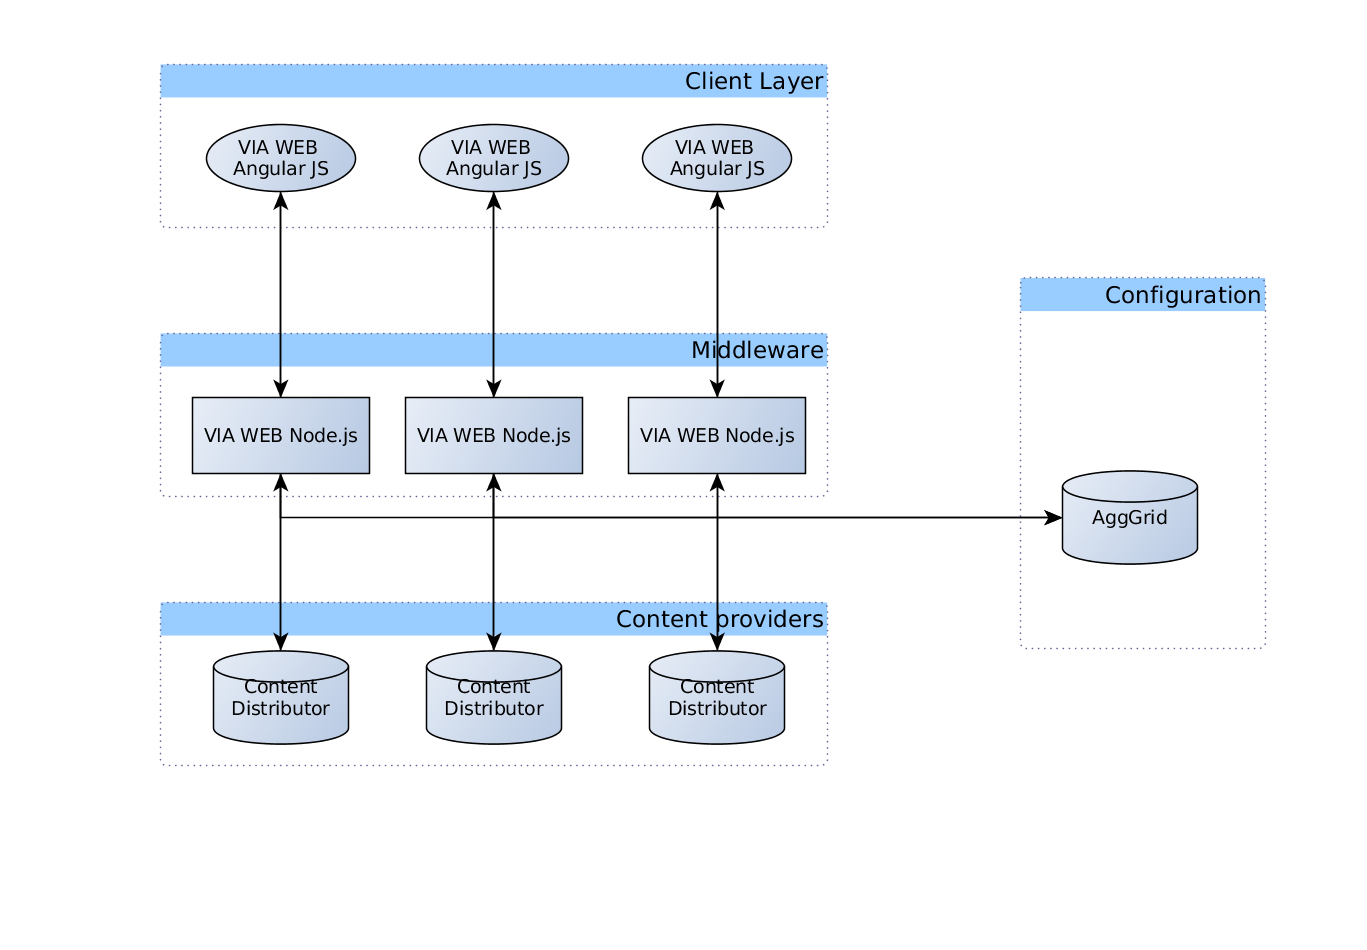
\includegraphics[width=\textwidth]{images/thesis_global_architecture_existing.png}
    \caption{Global architecture overview}
    \label{fig:arch_overview}
\end{figure}


The WEB Angular.js is a web application developed using Javascript, HTML, CSS framework and Model View Controller pattern. In the system, it is indicated as a client application. It communicates with the middleware server through REST services based on HTTP protocol. The client has several components: Controllers, Managers, and Services. 

The contollers validate the user data, invoke corresponding managers, and render data to the view objects represented by HTML pages. The managers are implemented using Facade pattern\cite{DesignPatterns}. They hold and manage services, construct View Model Objects from service responses, and send them back to the controllers. 

The services are the communication layer between the client application and the middleware server. They communicate via REST protocol based on HTTP protocol. This brings flexibility to the architecture and makes components loosely coupled.
% [describe why it is good?]. 

The WEB Node.js is a middleware server. It has several functions:

\begin{itemize}
	\item serves as a data aggregator and security point
	\item translates requests from the client application to the format understandable by the metadata server or content distributors
	\item gathers data from the content distributors
	\item builds data model objects and sends them as JSON entities to the client application.
\end{itemize}

Content servers (content distributors) are customer servers. They are the main sources of information that need to be presented by the client application. They can be represented, for example, by the movie entities or music distributors.

The metadata server is the company-developed server that stores and processes auxiliary and configurational information. The requests can be: 

\begin{itemize}
	\item Data aggregation - required for analytical purposes
	\item User action logs 
	\item User settings - specific user settings, for example, watch history for movie entities
	\item Client and middleware configuration
\end{itemize} 

The interaction between components can be described as follows: the client application initiates the process by sending requests to the middleware server. The middleware server then redirects requests to the underlying servers (content distributors or metadata server), builds data model objects, and sends them to the client application. The client request can be one of two types, configurational or data demand. If the request is configurational, the middleware server redirects it to the metadata server; otherwise, it redirects the request to the content server. The middleware supports the local cache and caches every response that is not associated with the user session. The message diagram between architecture components is depicted on figure \ref{fig:arch_uml}.


\begin{figure}[h]
\begin{center}

	\resizebox{1.0\textwidth}{0.8\textwidth} {

	\begin{sequencediagram}
	\newthread[white]{cl}{Client}
	\newinst[1.7]{mw}{Middleware}
	\newinst{lc}{Local Cache}
	\newinst[1.9]{ms}{Metadata Server}
	\newinst[1.3]{cs}{Content Server}

	\begin{call}{cl}{First request}{mw}{Response}

		\begin{call}{mw}{Create new session}{ms}{Session ID}
		\end{call}

		\begin{call}{mw}{Cache Session}{lc}{}
		\end{call}

		\begin{call}{mw}{Get content locator}{ms}{URL}
		\end{call}

		\begin{call}{mw}{Cache Locator}{lc}{}
		\end{call}

	\end{call}

	\begin{call}{cl}{GET Request}{mw}{GET Response}
		
		\begin{call}{mw}{Check Local Cache}{lc}{}
		\end{call}

		\begin{sdblock}{alt}{if data in cache}
			\begin{call}{mw}{Send response to Client}{cl}{}
			\end{call}
			\begin{sdblock}{else}{}
				\begin{call}{mw}{Request Content}{cs}{Response}
				\end{call}
				\begin{call}{mw}{Cache content}{lc}{}
				\end{call}
			\end{sdblock}
		\end{sdblock}


	\end{call}

	\end{sequencediagram}
	}

\end{center}
\caption{Sequence Diagram of message exchanging}
\label{fig:arch_uml}
\end{figure}

\subsection{Model objects}

In order to understand the existing architecture several definitions should be introduced: Data model object, View Model Object and Application model object.

The data from the content servers differ from one another; as a result, the structure for representing content server objects should be generated dynamically. The asset from the content distributor that has a dynamic structure is called \textit{Data Model Object}(DMO). For example, the DMO can represent information about videos, music, or any other entities. The DMO is generated by the DMO builders from JSON by the middleware server.

The middleware server sends DMOs to the client application. The client application gathers several DMOs and constructs a \textit{View Model Object}(VMO). This object is then presented to the users as a view asset. As a result, the VMO can be defined as a set of data model objects. The VMO is constructed for each HTML page. 

Each content distributor has a set of assets called \textit{Application Model Object}(AMO). Therefore, the application model object is the array of View Model Objects. The AMO represents the information and objects that can be fetched from the single content server.


\subsection{Middleware server architecture}

The middleware server is developed using server side Javascript language and asynchronous server Node.js \cite{Nodejs}. The server is developed using Model View Controller (MVC) pattern and communicates with other components through REST services. As a result, the server components are loosely coupled with each other which gives great flexibility in changing and replacing components and simplifies testing. 

The middleware contains the following components: Controllers, Managers, Services, Configuration and Data Model Object builders. The interraction between components is presented in figure \ref{fig:ms_req}.

\begin{figure}[h]
\begin{center}

	\resizebox{1.0\textwidth}{0.7\textwidth} {

	\begin{sequencediagram}
	\newthread[white]{cl}{Client}
	\newinst[1.7]{cntr}{Controller}
	\newinst[1.3]{mgr}{Manager}
	\newinst[1.3]{lc}{Local Cache}
	\newinst[1.3]{serv}{Service}
	\newinst[1.3]{es}{External Server}

	\begin{call}{cl}{Configuration request}{cntr}{Response}

		\begin{call}{cntr}{Invoke configuation manager}{mgr}{Response Data}
			\begin{call}{mgr}{Check Session key}{lc}{Cache Response}\end{call}
			\begin{sdblock}{alt}{if session key not in cache}
				\begin{call}{mgr}{Get session key using UUID}{serv}{Session key}
					\begin{call}{serv}{Session key request}{es}{Server response}
					\end{call}
				\end{call}
			\end{sdblock}
			\begin{call}{mgr}{Call data service}{serv}{JSON Data}
				\begin{call}{serv}{Call REST API}{es}{JSON data}
				\end{call}
			\end{call}
			\begin{call}{mgr}{Cache response}{lc}{}
			\end{call}
			\begin{call}{mgr}{Make DMO}{mgr}{DMO}\end{call}
		\end{call}

	\end{call}

	\end{sequencediagram}
	}

\end{center}
\caption{Sequence Diagram of Middleware Server Request Process}
\label{fig:ms_req}
\end{figure}

The controllers accept requests from clients. They validate user data and invoke corresponding managers.

The middleware server managers are similar to the client application managers: they implement facade pattern, aggregate multiple services, and redirect requests to them. They also gather the data from services and build immutable Data Model Objects (DMOs). These DMOs are sent back to the client as responses. The workflow of managers is depicted in figure \ref{fig:via_manager}.

\begin{figure}[h]
    \centering
	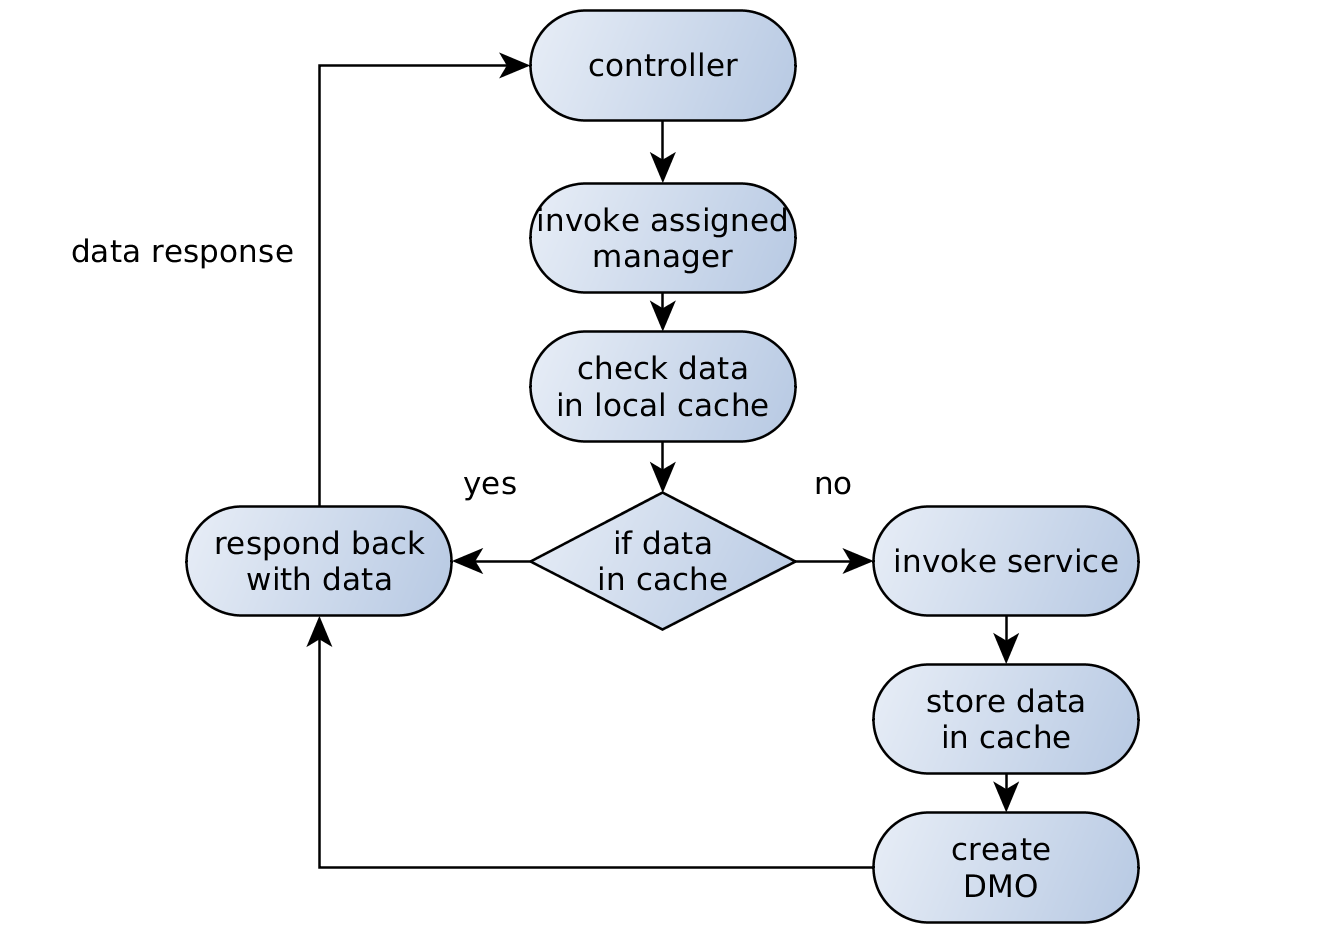
\includegraphics[width=\textwidth]{images/via_manager_1.png}
    \caption{Manager workflow}
    \label{fig:via_manager}
\end{figure}

The middleware services communicate with metadata and content servers. They aggregate the cache layer and react according to the following algorithm: first they check if the data is presented in the local cache; if the service observes cache hit, it will check the object's time to live (TTL) and send the corresponding object back to the manager. On the other hand, if a cache miss occurs, it will send the GET request through the REST protocol to the metadata server or content server, store the response locally for predefined period of time, and send it back to the manager. The workflow of services is presented in figure \ref{fig:via_service}. The time to live is the time (usually specified in seconds) that represents how long the object can be considered fresh without hitting persistence layer.


\begin{figure}[h]
    \centering
	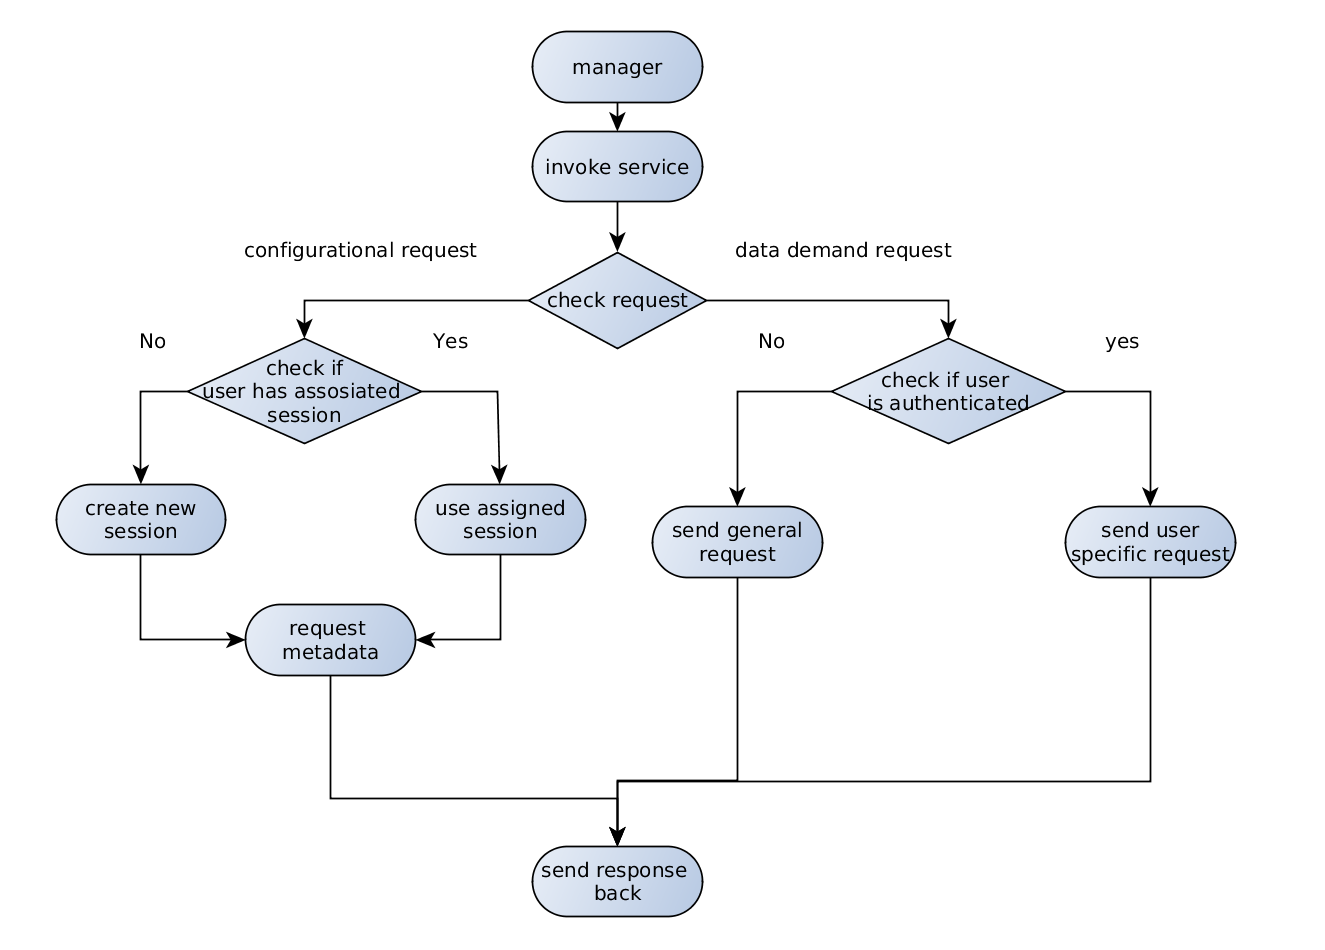
\includegraphics[width=\textwidth]{images/via_service_1.png}
    \caption{Service workflow}
    \label{fig:via_service}
\end{figure}


The client application can make two types of requests: configurational and data demand requests.
The configurational request can have the following purposes:

\begin{itemize}
	\item Provide configuration parameters for both middleware server and client application
	\item Write user activy
	\item Check the health of metadata server
	\item Get Content Server url
	\item User settings and preferences
	\item Analytics
\end{itemize}


The data demand request is a request to the content servers. Since content servers are customer servers, the response doesn't have predefined structure and can have any structure specified by customer service. 

The control flow can be described as follows: the controller receives a request from the client application, validates the data in the request, and redirects it to the assigned manager. The middleware server manager invokes the corresponding service (for example, communications layers). When the client application makes a data demand request, the manager invokes content service that redirects the request to the assigned content server. The response is then stored in the cache, translated into Data Model Object, and transferred back to the client in JSON format. The DMO builders are in charge of translating JSON data into persistent Data Model Objects. For every DMO, there is an assigned manager and service. For example, if the content server responds with a video object, there will be VideoManager and VideoService components.

\subsection{Session management}

The security layer, which is represented by the session management, is responsible for a communication process between the middleware server and inner servers (metadata server and content distributors).

The application session consists of two parts: 

\begin{itemize}
	\item client session
	\item middleware session
\end{itemize}

The purpose of sessions is to distinct between users and provide corresponding analytics to the customers.

The client session is represented by the unique session identifier (UID) and the browser's ID (the string that identifies browser version in the internet). These parameters are generated by the middleware server and transferred to the client through the \textit{set-cookie} header. The browser remembers the data and sends it back with every request in the \textit{cookie} header.


The session is generated per client when he makes the initial request. It contains the metadata session key and the user session, if the user is authenticated. The metadata session is obtained by making a request to the metadata server. The middleware server sends the application key parameter, which is specified in the configuration file and browser ID. The metadata server validates the application key and generates a new session for the middleware server. The middleware server assigns this session to the client and stores it in local memory. The client sends the unique session with each request to the middleware server. The middleware server retrieves the metadata session from the client's request. Using this session, the middleware server can make configurational requests to the metadata server. The sequence diagram of session management is presented in figure \ref{fig:arch_sess_uml}. The application key is given by the system administrator to each middleware server. The browser ID can be any string and does not have validation rules.

\begin{figure}[h]
\begin{center}

	\resizebox{1.1\textwidth}{0.5\textwidth} {

	\begin{sequencediagram}
	\newthread[white]{cl}{Client}
	\newinst[1.5]{md}{Middleware server}
	\newinst[3.0]{mt}{Metadata server}

	\begin{call}{cl}{RequestSession}{md}{Client session}

		\begin{call}{md}{GenerateSessionId}{md}{ClientSessionId} \end{call}
		\begin{call}{md}{GenerateBrowserId}{md}{BrowserId} \end{call}
		\begin{call}{md}{RequestMetadataSession}{mt}{MetadataSession} 
			\begin{call}{mt}{Validate Data}{mt}{}\end{call}
		\end{call}

	\end{call}

	\end{sequencediagram}
	}

\end{center}
\caption{Sequence Diagram of Middleware Session generation}
\label{fig:arch_sess_uml}
\end{figure}


\subsection{Drawbacks of the current architecture}

After careful examination, two categories of problems were defined: client application drawbacks and middleware server drawbacks. 

In order to render the page, the client needs to generate a view model object. The VMO contains several data model objects. The client makes a request for every DMO, aggregates the response, generates VMO from DMOs, and renders it to the HTML view. The drawback is that the client has to make several HTTP requests in order to generate a single VMO. It would be better for the client to make a request for VMO instead of DMO. This approach has some advantages: the client will make less HTTP requests which will increase the performance by reducing the latency and simplify the client's logic considering the client will not be required to generate VMOs from DMOs. 

Another problem with the current client implementation is that it is not generic. If a new content server is introduced, a lot of code would have to be modified on the client side in order to implement the new logic. To solve this, the client can maintain the caching layer that will cache VMOs from the responses. 

Additional complications occur when the client implements MVC pattern, which produces duplication with the middleware server. This approach increases the complexity of the system, since the developers would have to support both the client and the middleware MVC applications. To rectify this, we can simplify the client application and assign two tasks to it: caching and rendering VMOs.

On the middleware side, the DMOs are not generic. The purpose of the middleware server is to serve as a transparent layer, but without dynamic DMO generation a lot of code has to be changed when the new content server is introduced.

The middleware cache can be replaced by the Content Delivery Network (CDN). The middleware caches only information that is common for every user. This work can be done by the CDN edge servers. These will decrease the middleware complexity and decrease the cost of maintaining middleware server.


\newpage

\section{Model and Methodology}

The next two chapters describe the methodology and proposed solutions to improve the performance of the current company middleware server. In particular, the model consists of three parts: replacing the Redis cache server with web cache solution, reducing the amount of requests for generating view model objects, and removing duplication of the MVC pattern. This section describes the solutions for replacing Redis cache and the next section describes the algorithm for reducing requests to the middleware server and removing duplication.

\subsection{Reversed proxy cache}

The figure \ref{fig:req_amount} shows the amount of requests and time that the browser needs in order to generate a single VMO and render a page. The browser needs to make more than twenty AJAX requests for a single page. The middleware was deployed on the local machine meaning there is no latency between the browser and the middleware server. As can be seen, these are not optimistic numbers. The amount of requests are too high and computation has to be done on the both client and server sides. Several questions arise:

\begin{itemize}
	\item Is Redis a good caching layer for this project?
	\item Can Redis be replaced by something else? Maybe it would be better to use the configurational cache (represented by the web caches) and control it through the HTTP cache control headers?
\end{itemize}


\begin{figure}[h]
    \centering
	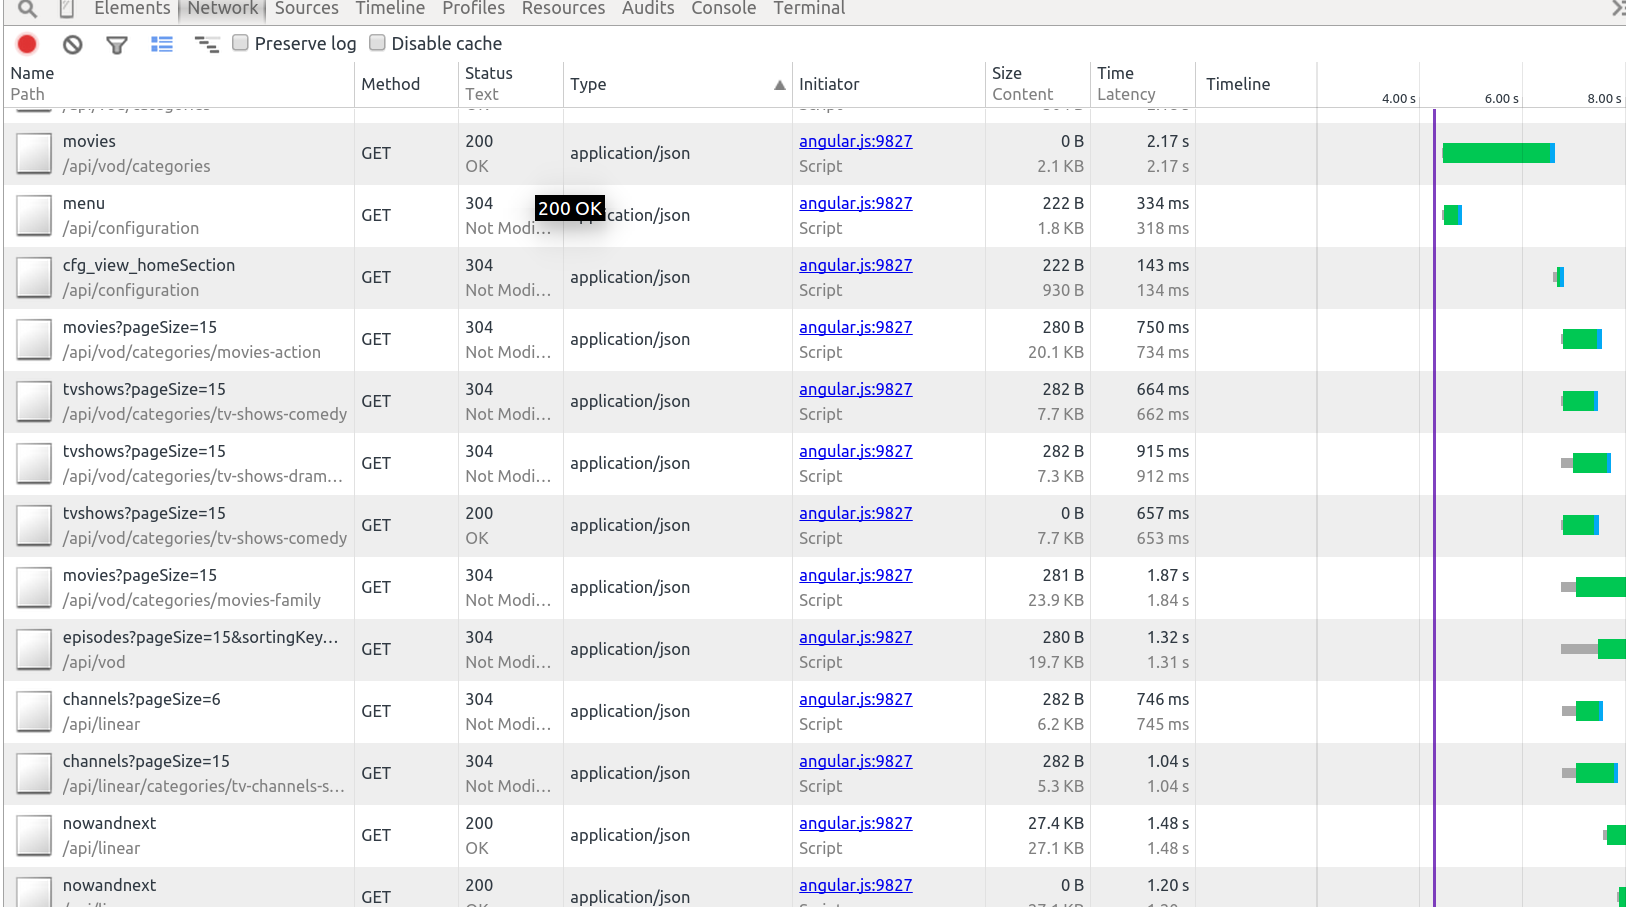
\includegraphics[width=\textwidth]{images/amount_of_requests.png}
    \caption{Example of page generation by the browser}
    \label{fig:req_amount}
\end{figure}

Let’s consider a system architecture using reversed proxy server instead of Redis cache. In this case, the client application makes HTTP requests through the reversed proxy server. The proxy server decides whether the content is stale or not and acts as a web cache: if the content is stale (non-cacheable) the proxy server redirects the request to the middleware server; Otherwise, it replies to the client application without touching the middleware server. The benefit of this solution is that instead of contacting the server and then caching the object, the cache is contacted before the server. In theory, the approach should give performance and flexibility. The Redis cache could be replaced by the Content Delivery Network solution in future.

% describe your solution on the top level

\subsection{Web cache selection}

The web cache for the project should satisfy several parameters:
\begin{itemize}
	\item Be Configurable- The client application sends requests both for DMOs and for writing user actions. The web cache should not cache the requests when writing user actions. However, the session should still be supported in order to write user actions. 
	\item Be Responsive, Easily Maintainable- The web cache should be deployed easily and provide statistics and internal logging. 
	\item High performance- The web cache should be transparent and must not increase the request time and latency if the cache object is not found locally. 
	% todo add more criterias
\end{itemize}

There are many web cache solutions available in both commercial and open source markets. For this project, only open source solutions were considered. The initial candidates were: Squid, Varnish, Apache server with proxy module, Nginx server as a cachable reversed proxy, and Apache Traffic Server.

The Squid server is a forward proxy server, but it can be configured as a reversed proxy server. Squid is preferably used for storing static content.

The Varnish was developed as a reversed proxy server from the beginning. It is fast, reliable, and lightweight. It uses Varnish Configuration Language (VCL) for configuring and describing the data workflow in cache. The VCL is translated into the C code and compiled to a shared object which is then dynamically linked into the server process. It is a powerful tool that helps to set up Varnish as a dynamic reverse proxy server.

The Apache Traffic Server was developed by the Yahoo group and eventually moved to the Apache Incubator \cite{GuApacheTrafficUri}. According to Yahoo Inc., the Apache Traffic Server can handle more than 400TB of internet traffic per day and works as a forward as well as a reversed proxy server. It has a growing community and is continously improved upon. The configuration is simple and consists of changing several files. All these make the Apache Traffic Server a good candidate.  

Other solutions (Nginx and Apache server) were not originally developed to be proxy servers, but have additional modules that one can install and configure. However, they are not well-configured and work worse than the solutions described above \cite{GuApacheTrafficUri}.

A thorough comparison and performance evaluation of Varnish and Apache Traffic Server can be found in \cite{VarnApacheReverse}.    

%TODO make a benchmarking analysis of the open web proxy caches
%TODO update the report, insert thate results about benchmarking and selection

\subsection{Web cache configuration}

Before performing an execution and comparative study, reversed proxy servers should be properly configured. They should aggregate and store requests that contain public data and skip analytical requests and requests with private user information. For example, payments.

Proxy servers should also work with HTTP sessions. Usually, when the session is specified (the \textit{set-cookie} HTTP header included in the server response), proxy servers are transparent, meaning they are skipping these requests and not storing them in memory. As was described in previous chapters, the metadata server uses HTTP session for analytical purposes. This means that even anonymous users will have a unique session. 

In order to solve this problem, the Varnish was configured to replace \textit{cookie} header with \textit{x-cookie} header. This gives the possibility for Varnish to store the requests and still have the analytical requests available. The metadata server was modified in order to treat \textit{x-cookie} header as a \textit{cookie} header.   

\subsubsection{Varnish configuration}

The varnish logic is configured using Varnish Configurational Language(VCL). The varnish logic works as a deterministic state machine consisting of several states:

\begin{itemize}
	\item vcl\_init -- the initial state 
	\item vcl\_recv -- the initial point for the request to varnish
	\item vcl\_pass -- in this state the request is passed to the backend server
	\item vcl\_hash -- the varnish computes the hash of the request in this state
	\item vcl\_hit -- occurs when the hit is observed on varnish server
	\item vcl\_miss -- occurs when varnish has stale data or has no data at all
	\item vcl\_fetch -- when the document is acquired from the backend server
	\item vcl\_deliver -- when the cache object is about to be delivered to the client
	\item vcl\_error -- occurs when the error is observed
\end{itemize}

The Varnish configuration is presented in Appendix A.

The Varnish server starts from the command line with the appropriate arguments. The Varnish uses the following arguments:

\begin{itemize}
	\item -a : the backend server address in format ADDRESS:PORT
	\item -b : the  address in format ADDRESS:PORT
	\item -f : the path to the VCL file 
	\item -F : if specified, the varnish will be started in the foreground
	\item -n : the varnish working directory
\end{itemize} 

\subsubsection{Apache Traffic Server configuration}

The Apache Traffic Server configuration consists of several files: 

\begin{itemize}
	\item cache.config -- the caching behaviour is specified here
	\item remap.config  -- is used for overall configuration
	\item cluster.config -- is used for configuring Apache Traffic Server in distributed mode
\end{itemize}

The Apache Traffic Server uses the command line to start. The obligatory parameter is --HTTP port which specifies the listen port. The Apache Traffic Server consists of three parts:

\begin{itemize}
	\item traffic\_cop -- supervises process for traffic\_server 
	\item traffic\_manager -- monitors the traffic\_server and gathers the logs
	\item traffic\_server -- responsible for starting the web cache server
\end{itemize}

The detailed configuration can be found \cite{ats_site}

\newpage
\section{Hierarchical VMO Generator}

\subsection{View model objects}

% introduction
The company's solution was developed in order to provide flexibility and customisation to the end user. The middleware server retrieves all configuration from the metadata server. The configuration can be user specific information as well as global information e.g. the location of content distributors. The middleware translates the responses from the content distributors to Data Model Objects. They are the immutable objects that are transferred to the client's application. On the other hand, the client application operates with View Model Objects. They are used to reder HTML pages. Single HTML page can contain single View Model Object. The VMO is constructed from mutliple data model objects and some additional information(e.g. the location of the image).   

One important drawback could be noticed: application dublication. The middleware server and the client application have the same pattern of execution: they both operate with data and build new data patterns from existing ones. The difference is that the middleware server is doing it with content distributor responses and the client aplication is processing middleware responses. Because of this situation, the client application should make several HTTP requests for retrieving necessary DMO objects from the middleware server.  The example of the single page generation is on the picture \ref{fig:vmo_example}. As can be seen, in order to generate a single main page, the client application has to make about ten Ajax requests. What, if there was a possibility to generate the VMO objects on the middleware side?  Maybe, there would be a possibility to get rid of the dublication? What should be done for it? This section will describe the solution for removing dublication of MVC pattern and reducing the amount of requests to the middleware server. 

\subsubsection{VMO properties}

% describe examination of applications(Algar, RTelecom, ViaWeb)

Typical DMO and VMO objects are presented in appendix E. As could be noticed a VMO object is a JSON dictionary build from DMO objects. The VMO supports following properties:

Generic. The DMO objects are specific and unique for every content distributor. They are build according to the specific rules in the middleware server. The VMOs are generated from DMOs according to another set of rules specified in the client application. As a result in order to move VMO generation to the server side some descriptive language should be introduced that lets developers to describe the VMO structure.

Hierarchical. DMOs are basically data from content distributors. That means that the DMOs can be depend on other DMOs. For example, the figure [add DMO dep. figure] shows that in order to build a movie list DMO, first the DMO that represents movie categories should be generated, than for each movie category, the set of movie objects should be fetched, and only on the third step, the list of movies could be build. These means that the VMOs have a hierarchical structure. The typical VMO is presented on figure \ref{fig:vmo_example}.

\begin{figure}[h]
    \centering
	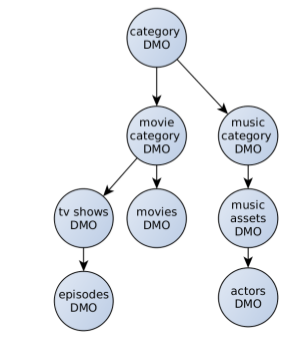
\includegraphics[width=8cm,height=10cm,keepaspectratio]{images/vmo_example.png}
    \caption{VMO from the set of dependant DMOs}
    \label{fig:vmo_example}
\end{figure} 

\subsection{Suggested Middleware server architecture}

In the current architecture, the single instance of the middleware server is deployed for a single content distributor. This is done due to the specifics of content distributors and data that they are providing. The question arises, is there a possibility to move the individual logic that requires to processes data to the client application while keeping the middleware as generic as possible? The theoretical benefits of this approach are: there will be needed single middleware server or cluster deployed. It will simplify the deploying system: instead of supporting middleware for every content distributor, there will be just one. The new architecture is presented of figure \ref{fig:arch_overview_new}. As can be seen, the configuration server(Appgrid) is now treated like a content distributor. The benefit is that we do not need specify separate logic for it. 

\begin{figure}[h]
    \centering
	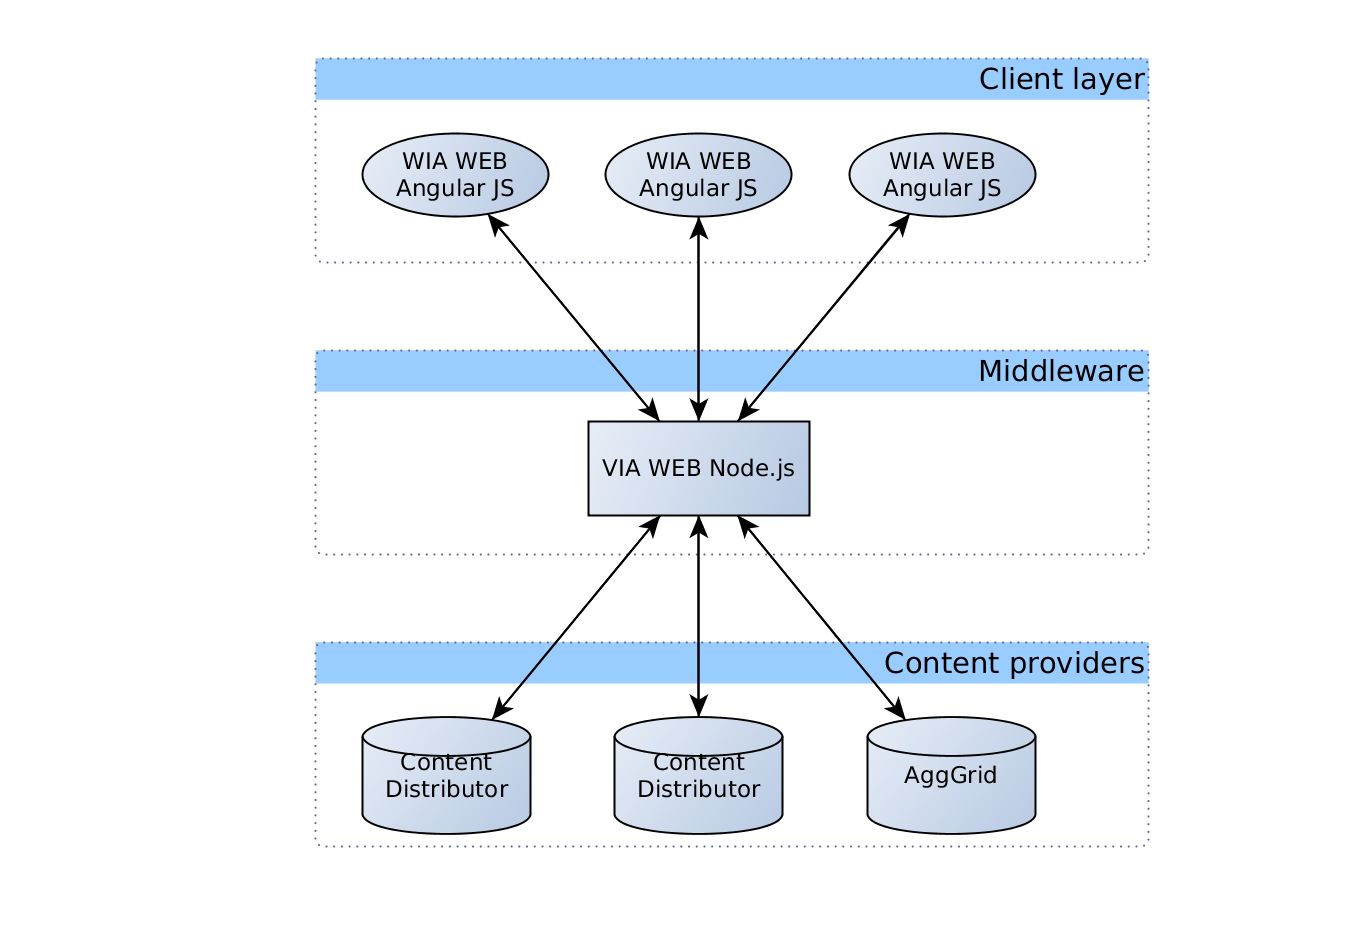
\includegraphics[width=\textwidth]{images/thesis_global_architecture_new.png}
    \caption{Manager workflow}
    \label{fig:arch_overview_new}
\end{figure}

Lets consider the architecture from another prespective.
The middleware server receives queries for the VMO generation. It supporsts several content distributors(databases), it makes queries to the content distributors for retrieving data model objects(tables). The middleware server resembles a lot a relational database system. The comparison of database management system and middleware server is presented on figure \ref{table:db_ms}

\begin{table}
\begin{center}
  \begin{tabular}{||p{3in}|||p{3in}||}
    \hline
    Database & Middleware server VMO generation  \\ \hline
    serves multiple clients & should serve multiple client applications  \\ \hline
    supports creation of new databases & should support insertion of new content servers  \\ \hline
    supporst creation and alternation of tables & should support creation and alternation of new endpoints  \\ \hline
    supports dynamic queries to the desired databases and tables & should support queries to the content distributors and theis endpoints \\ \hline
    \hline
  \end{tabular}
  \caption{Comparison of Database Sysem and Middleware Server properties}
  \label{table:db_ms}
\end{center}
\end{table}

\subsection{Approach description}

Let's consider relational database management systems and applications that are using them. There is usually a single instance or cluster of databases insalled and deployed on servers, depending on the amount of requests it should serve. Nobody makes new database instance for a single client, because it is neither efficient nor effective. In order to get data from the database the queiries are executed. The SQL queries are basically the rich descriptive language that is interpreted by the database and executed for specified tables. The data is provided in two forms: array of table rows and array of view rows. Tables are the single source of information that resembles a lot DMO. Views are the mixed information from tables that looks like VMO. 

In order to solve the problem of dublication and reduce the amount of requests, the hierarchical VMO generator(HVG) was developed. The HVG basicaclly the descriptive language, that developers are writing in a JSON format. The json is then translated into the GET HTTP or POST HTTP request and sended  to the middleware server. The middleware server parses the request, builds the asyclic graph and fetches the corresponding data model objects. The data model objects then combined together and sended as a response to the client application. The client application executes specific logic on the data received from server and builds HTML pages.

% The picture [insert picture] describes the VMO 

% picture of DBMS and Middleware server
% picture of DBMS tables and queries to the middleware server

\subsection{Path in VMOs}

This section introduces the definition of path in the View Modelw Object. The main format for data transferring is JSON. The JSON format consists of two main objects: array and dictionary. The example of dictionary:

\lstset{ %
    caption=The example of JSON dictionary,
    basicstyle=\ttfamily\footnotesize\bfseries,
    linewidth=0.6\textwidth
 }
\begin{lstlisting}[linewidth=5cm]
	{key1:value1,key2:value2,key3:{key1:value1}}
\end{lstlisting}

 
The example of array: 

\lstset{ %
    caption=The example of JSON array,
    basicstyle=\ttfamily\footnotesize\bfseries,
    linewidth=0.6\textwidth
 }
\begin{lstlisting}
	[value1,value2,value3:{key1:[value1,value2]}]
\end{lstlisting}

Very complex entities can be built using combinations of these two objects. Let's introduce the definition of path: The path is the route to the specific object or a set of objects in a JSON entity. 
The examples of path are presented below:
\lstset{ %
    caption=The examples of objects in different routes,
    basicstyle=\ttfamily\footnotesize\bfseries,
    linewidth=0.6\textwidth
 }
\begin{lstlisting}[linewidth=5cm]
	Object: {root:{child:value}}
	Path: root.child
	Value: value

	Object: {root:[{key:key1, value: value1},{key:key2,value:value2}]}
	Path: root.key
	Value: [value1,value2]

\end{lstlisting}


As can be seen, the path identifies a single object if it lays though a set of dictionaries. However, if the array is found on the route, all elements will be traversed and a set of objects will be extracted. 


\subsection{Hierarchical VMO Generator overview}

In order to solve the problem of multiple requests and middleware server dublication, the descriptive hierarchical VMO generator was implemented. It consists of three modules: HVG fetcher, HVG query parser and HVG query builder. In order to build and process VMOs two data structures are used: content provider dictionary and query dictionary. 

The content provider dictionary has a tree based structure and its scheme is presented on \ref{fig:content_provider_map}. Rectangles indicate the single instance of object appends parallelograms indicate the dictionary of objects. The content provider dictionary contains a dictionary of content distributors. When the query is passed to the middleware server, the locations of necessary content distributors are retrieved from this dictionary. It is uesd by the HVG fetcher module.

The key is a unique identifier that is used by query objects that are described below. Each content provider consists of two parts: location and a dictionary of resources. The location is a domain with corresponding scheme. The resource has one field: endpoint. The endpoint is a path in URI[RFC to URI] with several embedded templates. The template can be
one of two types: \textit{\{param\_id\}} and \textit{\{param\_id*\}}. The first type indicates that only one value can replace the template. If array of values is given, it will produce the array of resolved endpoints. On the other hand, the second type produces single endpoint, even if array of values is given. The examples of templates are presented in table \ref{table:template_replacement}.

% TODO: purpose

\begin{table}
	 \begin{center}
	  \begin{tabular}{l l}
	    Input values: & \textit{\{id:[value1,value2,value3]\}} \\
	    Endpoint: & \textit{http://testdomain.ext/\{id\}}  \\ 
	    Result: & [\textit{http://testdomain.ext/value1}   \\
	    		&  \textit{http://testdomain.ext/value2}   \\
	    		&  \textit{http://testdomain.ext/value3}]  \\
	    Endpoint: & \textit{http://testdomain.ext/\{id*\}} \\
	    Result: &  \textit{http://testdomain.ext/value1,value2,value3}
	  \end{tabular}
	 \label{table:template_replacement}
	 \caption{URL Template examples}
	\end{center}
\end{table}

The example of content provider map is given in Appendix C.


\begin{figure}[h]
    \centering
	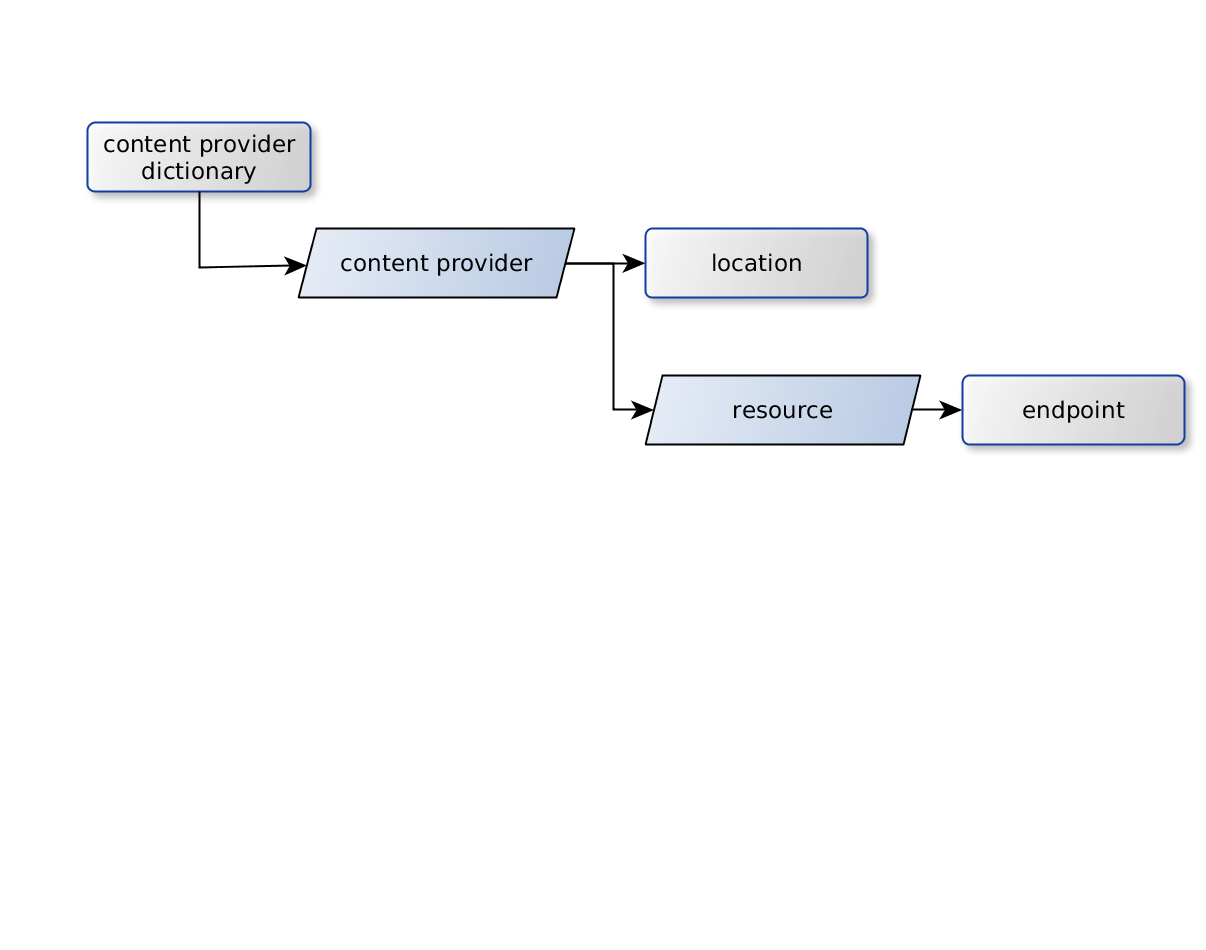
\includegraphics[width=\textwidth]{images/content_provider_map.png}
    \caption{Content Provider dictionary structure}
    \label{fig:content_provider_map}
\end{figure}


The query represents the request from the client application to the middleware server. The tree based structure is presented on figure \ref{fig:query_structure}. The single query consists of several query objects.

The query is built on the client application using HVG query builder. When the query is finished it is translated into corresponding JSON format and sent to the middleware server.

Each query object may have up to three parameters: \textit{content\_distributor}, \textit{path\_parameters}, \textit{query\_parameters}. The obligatory parameter, \textit{content\_distributor}, corresponds to the key in content provider dictionary desrcibed above. Through it the set of resources is retrieved from the content provider dictionary. The \textit{path\_parameters} and \textit{query\_parameters} are similar to each other, as a result only one of them will be described. The \textit{query\_parameters} is a dictionary of parameters, the key corresponds to the template parameter in resource object described above. Each path parameter has type field. It can have one of two values: \textit{constant} or \textit{dependency}.If the value is \textit{constant}, only one additional field should be specified: \textit{values}. This field serves as a container of values that should replace the corresponding template in the endpoint. 


On the other hand, if the value of \textit{path\_parameter} is \textit{dependency}: the query object depends on another query object e.g. for getting the list of movies from the content distributor, the list of categories should be requested first. That means that in order to request a query object, the parent object should be requested first and specified dependency variables for template parameters should be retrieved. In this case, additional parameters should be specified: \textit{parent}, \textit{parent\_parameter\_type}, \textit{path} and \textit{property}. The \textit{parent} specifies the query object identifier of the parent object. The \textit{path} is a JSON path to the object described above. The \textit{property} is a key in the dictionary retrieved by using \textit{path} parameter. The \textit{parent\_parameter\_type} can be one of two values: \textit{key} or \textit{constraint}. If the value is \textit{key} then the dependency variables will be extracted using path: \textit{path}+\textit{property}.

If the value of \textit{parent\_parameter\_type} is \textit{constraint} then the objects in \textit{path} that obey constraints will be retrieved. In this case, the additional parameter should be specified in corresponding path parameter: \textit{constraints}. The \textit{constraints} is an array of constraints. Each constraint has two parameters: key and value. The key specifies the name of the property that the object should have and the value specifies the value of the property. The summary of parameters is presented in the table \ref{table:query_obj_desrc}.


\begin{center}
	\begin{table}
	  	\caption{Description of Query Object's parameters}
	 	\label{table:query_obj_desrc}
	  	\begin{tabular}{|l|p{4in}|}
	    \hline
	    Parameter & Description  \\ \hline
	    content\_distributor & the location of resource dictionary in provider  \\ \hline
	    path\_parameters & dictionary of variables that will be retrieved in runtime and replace the corresponding template parameters in endpoint for building a request URL  \\ \hline
	    type & the type of path\_parameter, can be constant or dependency  \\ \hline
	    parent & the parent id of query object. Note: specified only when type=dependecny \\ \hline
	    parent\_parameter\_type & the parent parameter type, can be key or constraint. Note: specified only when type=dependecny \\ \hline
	    path & the path for the objects in parent response. Note: specified only when type=dependecny \\ \hline
	    property & the name of property that contains dependency value. Note: specified only when type=dependecny \\ \hline
	    constraints & the array of constraint. Note: specified only when type=dependecny  and path\_parameter\_type=constraint\\ \hline
	    \hline
		\end{tabular}
  	\end{table}
\end{center}


Hierarchical Query Parser(HQP) is a module that translates client requests into JSON format. The available methods are presented in table \ref{table:hqp_parameters}.

\begin{center}
	\begin{table}
		\label{table:hqp_parameters}
	  	\caption{Description of HQP module}
		\begin{tabular}{|l|p{1in}|p{3in}|}
	    \hline
	    Method Name & Parameters & Description  \\ \hline
	    select & object id, content distributor id & creates an empty query object with specified content distributor id  \\ \hline
	    setConstantParameter & parameter id, values & appends the path parameter which has a type \textit{constant} to the query object's path\_parameters dictionary  \\ \hline
	    setParentParameter & parameter id, parent query object, path , property & appends the parent parameter to the query object  \\ \hline
	    setQueryParameter & key, value & appends query parameter to the query objects query\_parameters dictionary \\ \hline
	    addConstraints & path parameter id, array of constraints& appends the constraint array to the query object's path patrameter \\ \hline
	    build & &  translates query objects into JSON format  \\ \hline
	    \hline
	  	\end{tabular}
  	\end{table}
\end{center}

The example of HQP usage is given in Appendix D.


\begin{figure}[h]
    \centering
	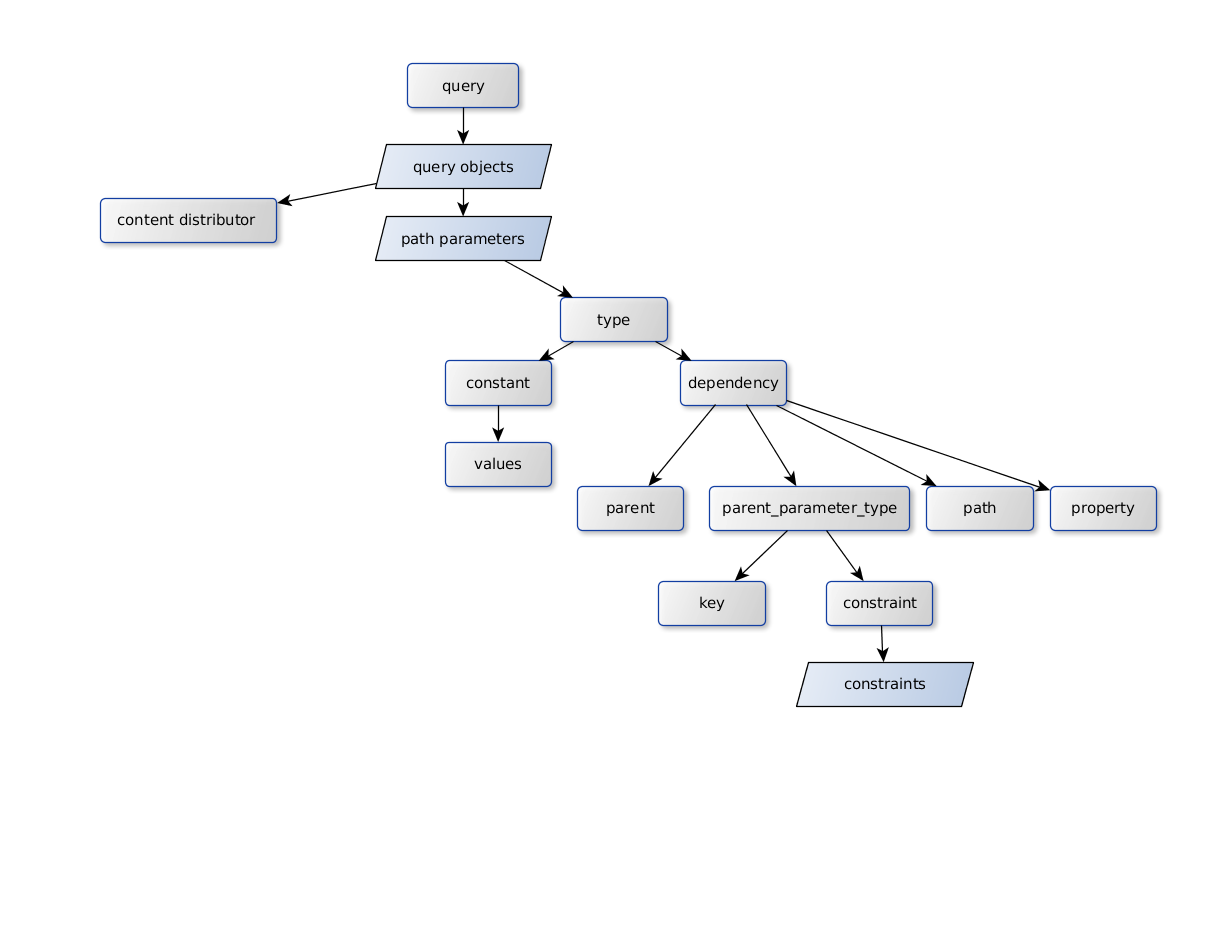
\includegraphics[width=\textwidth]{images/query_structure.png}
    \caption{Query structure}
    \label{fig:query_structure}
\end{figure}


The HQL supports two level caching. The first level caches the data model objects. It lays after parsing the client request strictly before requesting data from the content distributor. The second level cache lies on top of the execution process and is touched before executing the client request.  

% TODO: add section about asynchronous computation

\subsection{HQL workflow}

The developer writes the request using HQL parser methods. The request is translated into a JSON format that contains a dictionary of query objects. The JSON is sent as a POST HTTP request to the middleware server. The middleware server builds the asyclic graph (if there were dependency cycles it will generate error). The direct asyclic graph is then traversed using breath first search algorithm, on every node(query object) the data is fetched from appropriate content distributor (if the parent data has already been fetched) and is written into the output array. The output array is then sent as a response to the client POST request. 

The schematic workflow of HQL fetcher and HQL query parser is presented on fiqure \ref{fig:hvg_workflow}.

\begin{figure}[h]
	\begin{center}
		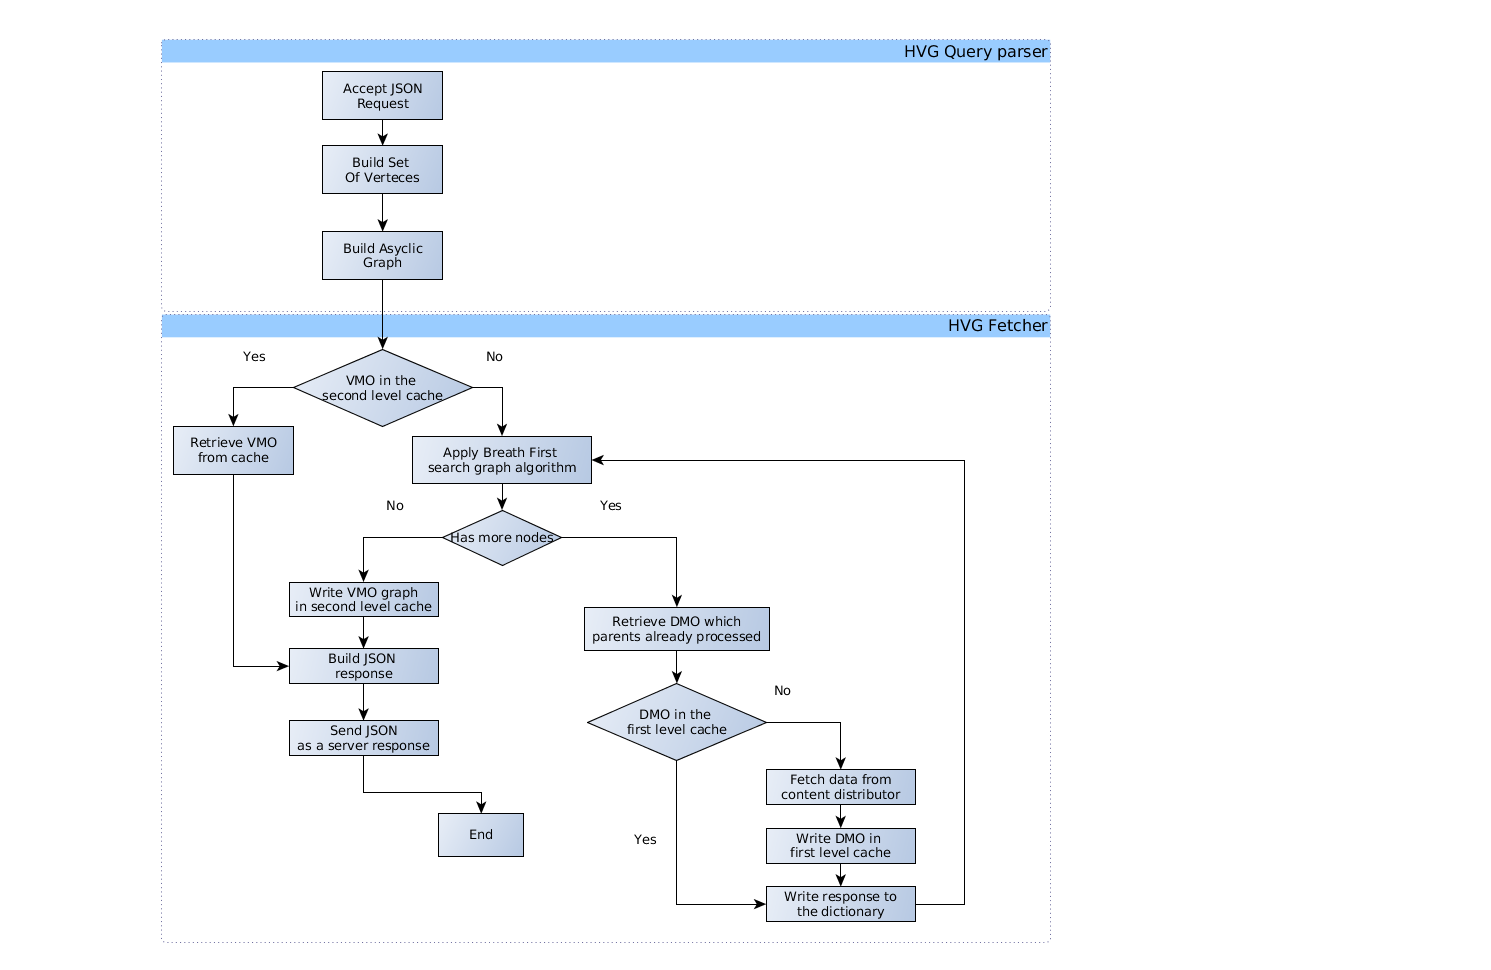
\includegraphics[width=20cm]{images/hvg_qp_workflow.png}
   		\caption{HVG workflow}
    	\label{fig:hvg_workflow}
	\end{center}
\end{figure}

\subsection{Alternatives to HVG}

The middleware server can be used in order to build one of three object types: Data model object, View model object or Application model object. The initial implementation was responsible for building DMOs. The current implementation builds the VMOs.

The DMO and VMO were described above. The Application Model Object(AMO) contains a set of VMOs that are specific for a content distributor. The alternative to the dynamic VMO generation on the middleware side can be generation of AMOs on the middleware server. Unfortunately, it is not a good idea, because the size of object provided by content distributors can
vary a lot and some of them can be very heavy. If the full AMOs would be transferred to the client application the big amount of memory should be utilized by both client application and middleware server. In theory, it will dramatically decrease the user experience, but it could be checked as a continuation to this project.


\newpage
\section{Testing}

Testing parameters:
1. Amount of requests per secong
2. Concurrent clients
3. Throughoutput
4. Code complexity
5. Supporting the solution
6. Time per requests

% according to what parameters did you test
% what are the testing criterias
% what type of tests do you need to make
% 

\subsection{Testing frameworks}

The following frameworks where selected for testing: Apache benchmark tool, Jmeter and Selenium. [urls for them]
The apache benchmark tool allows us to make load tests in order to understand what solution works faster and can serve more requests per second. It makes many concurrent requests to the single entity.

The Jmeter was selected in order to emulate the requests to the different pages. Because of the specific architecture of the middleware server and client application, in order to render single page client has to make several requests for getting DMOs. Using JMeter we can emulate users that are making requests to the different pages. 
% describe JMeter testing configuration
For each solution a single test plan was developed. The test plan emulates user requests to the resources. A single user request consists of the several requests for getting DMO objects. 

% describe what testing frameworks did you select and why

There are several types of proxy servers that can act as a reversed proxies.

Properties:
1. Availability
2. Configurational
3. Performance(amount of requests processed, memory usage)

Candidates:
Varnish
Squid in reversed mode
Apache in proxy mode
Nginx?

Benchmarking tools:
Apache benchmark testing tool
Jmeter

Use cases for requests: (selection of the optimal request/response headers for the dynamic and static contents)
1. LastModified and If-Modified-Since
2. Cache-Control: s-maxage, (public, private?, must-revalidate)
3. Etag and If-None-Match
4. Combination: Etag + LastModified
5. Combination: Etag + LastModified + CacheControl

Optimal for static content:
Optimal for dynamic content:


\newpage


% The most fundamental difference between Squid and Varnish is that Squid is forward proxy that can be a configured as a reverse proxy whereas Varnish is built from the ground up to be a reverse proxy.

% So, in principle Varnish is better suited than Squid to do reverse proxy HTTP. However, Squid is a very mature product and has had time to accumulate a lot of features that still are not available in Varnish. Both projects are used by huge websites and both of them can do almost anything.

% The main advantages of Squid over Varnish, as I see them, are:

%     Built in SSL support. Varnish needs stud, nginx or stunnel to do SSL.
%     Better support for Range and streaming delivery of objects.
%     Support for antivirus-plugins


% On the other hand, Varnish has:

%     An absolutely amazing configuration system. VCL gives unmatched flexiblity to run policies. Want to rewrite URLs coming from a certain user-agent requesting a specific URL coming from a specific network? Easy. With Squid, that configuration will be quite complex (if at all possible).
%     Better performance and scalability. Squid is a single process running on only one CPU core, whereas Varnish is threaded. Artur Bergman reported having a Varnish server serving 60K req/sec on real life traffic. That's more than most of us ever see and I doubt that you'll be able to see Squid push those kind of numbers.
%     Better and more flexible invalidation support. With Varnish you can invalidate content from cache based on more or less everything. I can elaborate on this.

Open Web caches:
Varnish
Squid
Apache proxy mod
Nginx

Measuring tools:
Jmeter
Apache benchmarking tool 


Squid: 
Forward proxy server, can be configured as a reversed proxy.
In order to cache less than 60 seconds, one should specify the cache-control headers (Last-Modified),
for dynamic objects it is quite hard to do. Even, if the Last-Modified was specified for cachanging for every request, squid will not make another request to server until s-maxage seconds pass.


Web cache as a load balancer:
Testing tool: apache benchmark 

Configuration:
Single request to the server through the varnish:
    ab -r -c 100 -n 1000    http://127.0.0.1:6081/
Redis turned on

Output: 

Concurrency Level:      100
Time taken for tests:   40.510 seconds
Complete requests:      1000
Failed requests:        0
Total transferred:      10177208 bytes
HTML transferred:       9614000 bytes
Requests per second:    24.69 [#/sec] (mean)
Time per request:       4051.013 [ms] (mean)
Time per request:       40.510 [ms] (mean, across all concurrent requests)
Transfer rate:          245.34 [Kbytes/sec] received

Connection Times (ms)
              min  mean[+/-sd] median   max
Connect:        0    1   2.0      0       8
Processing:   458 3681 652.4   3743    6194
Waiting:      458 3666 650.9   3728    6120
Total:        464 3682 651.2   3743    6194

Percentage of the requests served within a certain time (ms)
  50%   3743
  66%   3788
  75%   3806
  80%   3823
  90%   3889
  95%   4109
  98%   5417
  99%   5817
 100%   6194 (longest request)


Without web cache:

Concurrency Level:      100
Time taken for tests:   46.225 seconds
Complete requests:      1000
Failed requests:        0
Total transferred:      10105660 bytes
HTML transferred:       9614000 bytes
Requests per second:    21.63 [#/sec] (mean)
Time per request:       4622.455 [ms] (mean)
Time per request:       46.225 [ms] (mean, across all concurrent requests)
Transfer rate:          213.50 [Kbytes/sec] received

Connection Times (ms)
              min  mean[+/-sd] median   max
Connect:        0    0   0.8      0       4
Processing:   575 4435 1978.4   3787   11812
Waiting:      575 4435 1978.4   3787   11812
Total:        579 4435 1978.2   3787   11812

Percentage of the requests served within a certain time (ms)
  50%   3787
  66%   3839
  75%   3907
  80%   4411
  90%   7697
  95%   9467
  98%  10890
  99%  11237
 100%  11812 (longest request)



Without cache
Varnish 

...........................................................
net tests:
Test: ab -r -c 100 -n 1000    http://127.0.0.1:9000

Node.js+Redis: 

Concurrency Level:      100
Time taken for tests:   45.977 seconds
Complete requests:      1000
Failed requests:        0
Total transferred:      10105692 bytes
HTML transferred:       9614000 bytes
Requests per second:    21.75 [#/sec] (mean)
Time per request:       4597.743 [ms] (mean)
Time per request:       45.977 [ms] (mean, across all concurrent requests)
Transfer rate:          214.65 [Kbytes/sec] received

Connection Times (ms)
              min  mean[+/-sd] median   max
Connect:        0    0   0.8      0       4
Processing:  3618 4413 1725.6   3729   12484
Waiting:     3618 4413 1725.6   3729   12484
Total:       3618 4413 1726.1   3730   12486

Percentage of the requests served within a certain time (ms)
  50%   3730
  66%   3767
  75%   3808
  80%   3904
  90%   6803
  95%   8554
  98%  10907
  99%  11835
 100%  12486 (longest request)


cost
code complexity
amount of time

\newpage
\section{Discussion and Conclusion}
	
Several conclusions can be made using the results of previous chapter: 

\begin{itemize}
	\item The Hierarchical VMO Generator(HVG) works slower than company's solution without first level cache
	\item The stability of HVG depends on the amount of transferred data: the less data the more stable responses
	\item Without latency (that was introduced artificially) the HVG with optimal configuration works roughly with the same speed as current company solution where VMOs are generated on the client side
	\item With latency the HVG solution works faster 
\end{itemize}

The \cite{VarnApacheReverse} gives the detailed evaluation of Apache Traffic server and Varnish server; As a result, the comparison between them is omitted in this project. 

The HVG solution consumes more CPU and memory because it stores the graph of data model objects plus the fetched data from content distributors. It uses computationally intensive breadth first search algorithm on directed graph. On the other hand, the client side VMO generation sends multiple simple requests to the middleware server. They are light requests, that consume small amount of CPU power and memory and is used just for storing the final dta model object.

Fortunately, the algorithm for generating HVG is executed rarely because most of the time the data is retrieved in the VMO cache. The drawback of this approach is that the data is stored two times: one as a part of Data Model Object, another as a part of View Model Object. The Data Model Object cache could be turned off, unfortunately these will give additional problems: if the VMO will be stored for the time equals of maximum TTL among all DMOs, some DMOs will become stale and the server response will be irrelevant. Taking this in consideration, the maximum TTL for VMO is computed as:

\begin{center}
	\begin{math}M = \min_{1 \leq i \leq N} D_{i},\{i=1:N\}\end{math}, N - amount of DMOs that need to be fetched in request.
\end{center}

Theoretically, the solution with HVG does not work well when the set of DMOs have TTL that dramatically differs from one another. In this case, the overhead produced by VMO computation will be greater than the latency for retrieving data model objects, but in general it requires additional study. 

\subsection{Further studies}

The Application Model Object(AMO) should be studied and corresponding conclusions should be produced. For small VMOs, perhaps it would be more optimal to transfer compressed AMO.

The Web cache solution requires additional study in terms of selecting the appropriate algorithm for calculating TTL (time to live) of VMO/DMO objects. Currently the TTL is set to the default time that was not selected through careful study. The maximum time for VMO equals the TTL of DMO that has minumum value. This is one of the proposed algorithms, however this question is not studied enough and requires futher work.

\newpage

% \begin{thebibliography}{99}

% \bibitem{norvig06}
%   П. Норвиг, С. Рассел,
%   \emph{Искусственный интеллект: современный подход}, 2-е изд.
%   М.: Издательский дом ``Вильямс'',
%   2006.

% \bibitem{forsight04}
%   Д. Форсайт, Ж. Понс,
%   \emph{Компьютерное зрение. Современный подход}.
%   М.: Издательский дом ``Вильямс'',
%   2004.

\end{thebibliography}


\newpage
\bibliographystyle{amsplain}
\bibliography{mybib}
\newpage
\begin{appendices}

\chapter{Appendix A}
	 % \includecode{codes/default.vcl}
	 \lstset{basicstyle=\footnotesize\ttfamily}
	 \lstinputlisting[frame=single,linewidth=15cm,breaklines, caption=Varnish Configuration ]{codes/default.vcl}

\chapter{Appendix B}
	 
	\begin{figure}[h]
    	\centering
		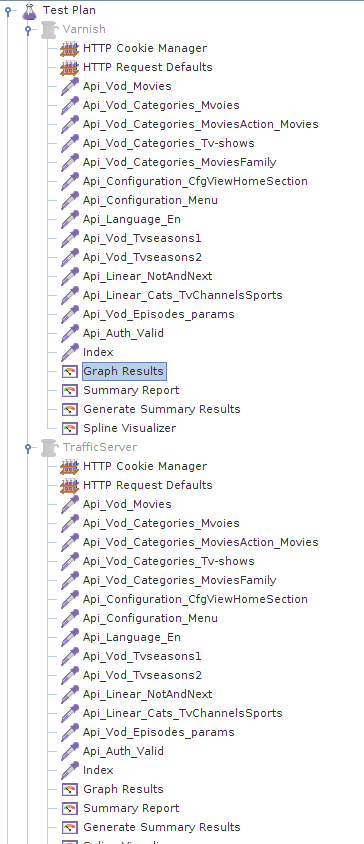
\includegraphics[width=10cm,height=15cm,keepaspectratio]{images/jmeter_conf.png}
    	\caption{Jmeter Configuration}
    	\label{fig:jmeter_conf}
	\end{figure}

\chapter{Appendix C}
	 % \includecode{codes/default.vcl}
	 \lstset{basicstyle=\footnotesize\ttfamily}
	 \lstinputlisting[frame=single,linewidth=15cm,breaklines, caption=Content Provider Dictionary ]{codes/content_provider.json}


\chapter{Appendix D}

\begin{lstlisting}[frame=single,linewidth=15cm,breaklines=true,caption=HQL usage]
	var parser = new HQLParser();
	var requestJson = parser
		  .select('category_movies', 'accedo.ovp.categories.movies')
		  .setConstantParameter('id', ['movies-action'])
		  .setQueryParameter('pageSize', 2)
		  .select('category_tvshows', 'accedo.ovp.categories.tvshows')
		  .setConstantParameter('id', ['tv_shows_comedy'])
		  .setQueryParameter('pageSize', 2)
		  .select('episodes', 'accedo.ovp.episodes')
		  .setQueryParameter('pageSize', 2)
		  .select('tvshow', 'accedo.ovp.tvshow')
		  .setParentParameter('id', 'episodes', 'entries.metadata', 'value')
		  .addConstraints('id', [{key: "name", value: "VOD$tvShowId"}])
		  .select('tvseason', 'accedo.ovp.tvseason')
		  .setParentParameter('id', 'episodes', 'entries.metadata', 'value')
		  .addConstraints('id', [{key: "name", value: "VOD$tvSeasonId"}])
		  .build();

\end{lstlisting}

\chapter{Appendix E}

\begin{lstlisting}[frame=single,linewidth=15cm,breaklines=true,caption=Example of VMO/multiple DMOs that were used for testing]
	 {  
   "movies_movies-action":{  
      "content_distributor":"accedo.ovp.categories.movies",
      "path_parameters":{  
         "id":{  
            "type":"constant",
            "values":[  
               "movies-action"
            ],
            "parent_parameter_type":"key"
         }
      },
      "query_parameters":{  
         "pageSize":{  
            "value":15
         }
      }
   },
   "tvshow    s_tv-shows-comedy":{  
      "content_distributor":"accedo.ovp.categories.tvshows",
      "path_parameters":{  
         "id":{  
            "type":"constant",
            "values":[  
               "tv-shows-comedy"
            ],
            "parent_parameter_type":"key"
         }
      },
      "query_parameters":{  
         "pageSize":{  
            "value":15
         }
      }
   },
   "tvshows_    tv-shows-drama-american":{  
      "content_distributor":"accedo.ovp.categories.tvshows",
      "path_parameters":{  
         "id":{  
            "type":"constant",
            "values":[  
               "tv-shows-drama-american"
            ],
            "parent_parameter_type":"key"
         }
      },
      "query_parameters":{  
         "pageSize":{  
            "value":1            5
         }
      }
   },
   "movies_movies-family":{  
      "content_distributor":"accedo.ovp.categories.movies",
      "path_parameters":{  
         "id":{  
            "type":"constant",
            "values":[  
               "movies-family"
            ],
            "parent_parameter_type":"key"
         }
      },
      "query_parameters":{  
         "pageSize":{  
            "value":15
         }
      }
   },
   "ep    isodes":{  
      "content_distributor":"accedo.ovp.episodes",
      "query_parameters":{  
         "pageSize":{  
            "value":15
         }
      }
   },
   "tvshow":{  
      "content_distributor":"accedo.ovp.tvshow",
      "path_parameters":{  
         "id":{  
            "type":"dependency",
            "parent":"episodes",
            "path":"entries.m    etadata",
            "property":"value",
            "parent_parameter_type":"constraint",
            "constraints":[  
               {  
                  "key":"name",
                  "value":"VOD$tvShowId"
               }
            ]
         }
      }
   },
   "tvseason":{  
      "content_distributor":"accedo.ovp.tvseason",
      "path_parameters":{  
         "id":{  
            "type":"dependency",
            "parent":"    episodes",
            "path":"entries.metadata",
            "property":"value",
            "parent_parameter_type":"constraint",
            "constraints":[  
               {  
                  "key":"name",
                  "value":"VOD$tvSeasonId"
               }
            ]
         }
      }
   },
   "channels":{  
      "content_distributor":"accedo.ovp.channels",
      "path_parameters":{  
         "id":{  
            "    type":"constant",
            "values":[  
               "tv-channels-sports"
            ],
            "parent_parameter_type":"key"
         }
      },
      "query_parameters":{  
         "pageSize":{  
            "value":15
         }
      }
   }
}
\end{lstlisting}

\end{appendices}



\end{document}


% -------------------------------------------------
% content
% 1. Introduction
% 1.1 Background
% 1.2 Project Objectives
% 1.3 Thesis outline
% 2. Theoretical part
% 2.1 Web Caching
% 2.1.1 Http Protocol
% 2.1.2 Cache Control in Http
% 2.1.3 Web Cache Layers
% 2.2 Content Delivery Networks
% 2.3 Server Side Caching
% 
% 3. Caching in Reversed proxies
% 3.1 Static Content
% 3.2 Dynamic Content
% 3.3 Architecture overview
% 3.4 Caching techniques
% 3.4.1 Time based caching
% 3.4.2 Data based caching
% 3.4.3 Comparison
% 3.5 Purging strategies for dynamic content

% 4. Server Side Caching
% 4.1 Server Caching strategies
% 4.2 Architecture overview
% 4.3 Content based caching
% 4.4 Cache eviction strategies

% 5. Results 
% 5.1 Reversed Proxy Caching
% 5.2 Server Side Caching
% 5.3 Comparison with existing middleware

% 6. Conclusion

% -------------------------------------------------

